\pagebreak

\section*{Anhang A}
\label{anhang_a}
\addcontentsline{toc}{section}{\nameref{anhang_a}}
Generell gehört alles Relevante in den Text. Irrelevantes wird weggelassen. Inhalte, die mit dem Thema in engem Zusammenhang stehen, aber nicht zwingend erforderlich sind, können in einen Anhang ausgelagert werden. üblicherweise gilt dies zum Beispiel für Herleitungen von Formeln oder umfangreiche Beweise, Quelltexte von Computerprogrammen oder umfangreiches (Daten-)Material, welches den Text überfrachten würde.

Wie Tabellen und Abbildungen müssen auch Anhänge im Text angesprochen werden und dürfen nicht losgelöst von diesem stehen.

\pagebreak


\section*{Anhang B}
\label{anhang_b}
\addcontentsline{toc}{section}{\nameref{anhang_b}}

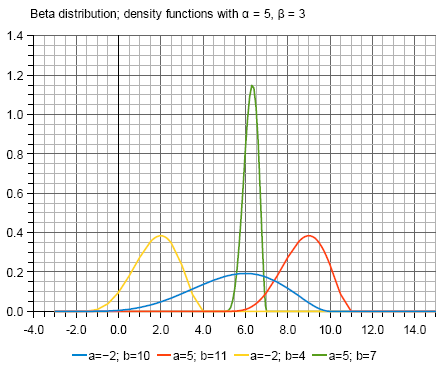
\includegraphics{source/img/graph.png}

\pagebreak
